\section{Experimenteller Aufbau}
\paragraph{meine Einstellungsparameter:}

\begin{itemize}
    \item Beschleunigungsspannung $U_B$ im Bereich von 12 kV bis 16 kV, zugehöriger Richtungsvektor $\vv{s} = \vektor{1}{0}{0}$
    \item Magnetfeldstärke zweier Ablenkspulen:
    
    \begin{itemize}
        \item $B_1$ im Bereich -5 mT bis 5 mT, zugehöriger Richtungsvektor $\vv{b_1} = \vektor{0}{0}{1}$ % senkrechte Spule
        \item $B_2$ im Bereich -5 mT bis 5 mT, zugehöriger Richtungsvektor $\vv{b_2} = \vektor{0}{1}{0}$ % waagerechte Spule
    \end{itemize}

\end{itemize}

\paragraph{Konstanten:}

\begin{itemize}
    \item Felddurchmesser $d$ = 30 in mm
    \item Masse des Elektrons $m$ =  $9,109 \cdot 10^{-31}$ in kg
    \item Ladung des Elektrons $e$ = $1,602 \cdot 10^{-19}$ in As
    \item Bildschirmabstand $l$ = 500 in mm
\end{itemize}

\paragraph{meine zu berechnenden Parameter:}

\begin{itemize}
    \item Teilchengeschwindigkeit v in $\frac{km}{s}$
    \item Ergebnisvektor $\vv{v}$
    \item Bahnradius r in mm 
    \item alpha $\alpha$
    \item Ablenkungsrichtung $\vv{a}$
\end{itemize}

\section{Berechnung der Elektronenkanone}

\section{Lorentzkraft und Ablenkung}

\section{Geometrische Bestimmung des Winkels}

\begin{tabular}{c|c|c}
     Formel Buch & Formel Block & Anmerkungen  \\
     \hline
    $\alpha = \frac{d}{r}$ &$\tan(\frac{\alpha}{2}) = \frac{d}{2\cdot r}$& wegen Kleinwinkelnäherung bei dem Buch \\
    \hline
   $r = \frac{m\cdot v}{q\cdot B}$  & $r = \frac{m\cdot v}{q\cdot B}$& alles gleich 
     
\end{tabular}


Das ist im Magneten und hier wird die Ablenkung berechnet.
\begin{figure}
    \centering
    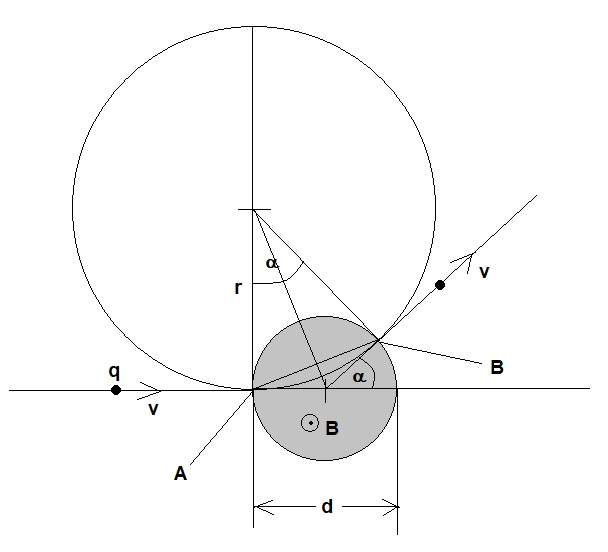
\includegraphics[width=.75\textwidth]{fig/elektronenstrahl-ablenkung_101.jpg}
    \caption{Skizze für Winkelberechnung}
    \label{fig:ausBlock}
\end{figure}

\paragraph{Die physikalischen Formeln:}

Wie wir in abbildung \ref{fig:ausBlock}.

\url{https://www.physikerboard.de/ptopic,342494.html#342494}

$$ r = \frac{m \cdot v}{e \cdot B}$$
$$ \tan(\frac{\alpha}{2}) = \frac{d}{2 \cdot r}$$
$$ \vv{a} = \vv{s} \cdot (-1) \times \vv{b}$$
\begin{lstlisting}
bahnradius
  = strahl.elektronenmasse
    * strahl.teilchengeschwindigkeit
    / (strahl.elektronenladung * magnetfeldstaerke/1000)
    * 1000;
alpha = 2 * Math.atan(felddurchmesser/ (2 *bahnradius ));
ablenkungsrichtung
  = strahl.quelle.richtungsvektor.
    multiplizieren(-1).
    kreuzprodukt(this.richtungsvektor);
\end{lstlisting}

Das ist im Strahl und hier wird die Geschwindigkeit berechnet mit welcher dieser aus der Elektronenkanone kommt. 

\textbf{physikalische Erklärung:}

Durch den glühelektrischen Effekt werden Elektronen freigesetzt. Dabei wird ein "Wehnelt-Zylinder" durch eine Heizspannung $U_H$ erhitzt. Die nun freien Elektronen werden durch die Kathode( positiver Pol) gebündelt. Dies geschieht dadurch das in der Mitte der Platte ein kleines Loch vorhanden ist durch welches der Elektronenstrahl nun fließt. Um die Geschwindigkeit zu bestimmen muss der Energieerhaltungssatz betrachtet werden. Dabei wird die kinetische Energie und die elektrische Energie gleichgesetzt. Um die elektrische Energie benutzen zu können, wird das Ende des "Wehnelt-Zylinder" als Anode aufgefasst( negativer Pol) und dadurch entsteht ein elektrisches Feld in welchem auch die elektrische Energie vorhanden ist. 
$$ E_{kin} = E_{el}$$
$$ \frac{1}{2} \cdot m \cdot v^2 = e \cdot U_B$$
Diese Formel wird  nun nach v umgestellt:
\paragraph{Die physikalische Formel:} 
$$ v = \sqrt{\frac{2 \cdot e \cdot U_B}{m}}$$

\textbf{Erklärung/ Umsetzung der Physik im Code:}

Im Folgenden ist der Code in der Simulation dargestellt. Zu sehen ist, dass die oben genannte Formel benutzt wird und die jeweiligen Attribute aus den zugehörigen Klassen geholt werden. Hier muss sich die Spannung $U_B$ aus der Elektronenkanone( quelle ) geholt werden. Des Weiteren wird die Spannung mit 1000 multipliziert, da in der Formel mit V gerechnet wird, während die Spannung der Elektronenkanone in kV angegeben ist. Deswegen muss diese noch umgerechnet werden.
\begin{lstlisting}
teilchengeschwindigkeit 
  = Math.sqrt(2 
  * elektronenladung 
  * quelle.spannung 
  * 1000 
  / elektronenmasse);
\end{lstlisting}

Hier wird der Punkt auf dem Bildschirm berechnet.

\textbf{Die physikalische Formel:}
$$ \vv{v} = \vv{v} + \vv{a} \cdot l \cdot \tan(\alpha)$$
\begin{lstlisting}
Vektor ergebnisvektor 
  = new Vektor(bildschirmabstand,0,0);
    for(Magnet m : getWorld().getObjects(Magnet.class) )
        {
            ergebnisvektor 
            = ergebnisvektor.addieren( m.ablenkungsrichtung.
            multiplizieren(bildschirmabstand).
            multiplizieren(Math.tan(m.alpha)));
        }
    return ergebnisvektor;
\end{lstlisting}
 
